\documentclass{article}

%other packages
\usepackage[a4paper]{geometry}
\usepackage{longtable}
\usepackage{wrapfig}
\setlength\parindent{0pt}
\usepackage{enumitem}
\usepackage[table,dvipsnames]{xcolor}
\usepackage{polynom}
\def\scaleint#1{\vcenter{\hbox{\scaleto[3ex]{\displaystyle\int}{#1}}}}
\usepackage{array}
\newcolumntype{C}{>{{}}c<{{}}} % for '+' and '-' symbols
\newcolumntype{R}{>{\displaystyle}r} % automatic display-style math mode 
\usepackage{tabularray}
\usepackage{dcolumn,tabularx,booktabs}
\usepackage[most]{tcolorbox}
\usepackage{tikzducks}


%maths
\usepackage{mathtools}
\usepackage{amsmath}
\usepackage{amssymb}
\usepackage{amsfonts}
\usepackage{autobreak}

%tikzpicture
\usepackage{tikz}
\usepackage{scalerel}
\usepackage{pict2e}
\usepackage{tkz-euclide}
\usepackage{tikz-3dplot}
\usetikzlibrary{calc}
\usetikzlibrary{patterns,arrows.meta}
\usetikzlibrary{shadows}
\usetikzlibrary{external}
\usetikzlibrary{decorations.pathreplacing,angles,quotes}

%pgfplots
\usepackage{pgfplots}
\pgfplotsset{compat=1.18}
\usepgfplotslibrary{statistics}
\usepgfplotslibrary{fillbetween}

\pgfplotsset{
    standard/.style={
    axis line style = thick,
    trig format=deg,
    enlargelimits,
    axis x line=middle,
    axis y line=middle,
    enlarge x limits=0.15,
    enlarge y limits=0.15,
    every axis x label/.style={at={(current axis.right of origin)},anchor=north west},
    every axis y label/.style={at={(current axis.above origin)},anchor=south east}
    }
}

\begin{document}
\topskip0pt
\vspace*{\fill}
\begin{center}
\resizebox{\textwidth}{!}{
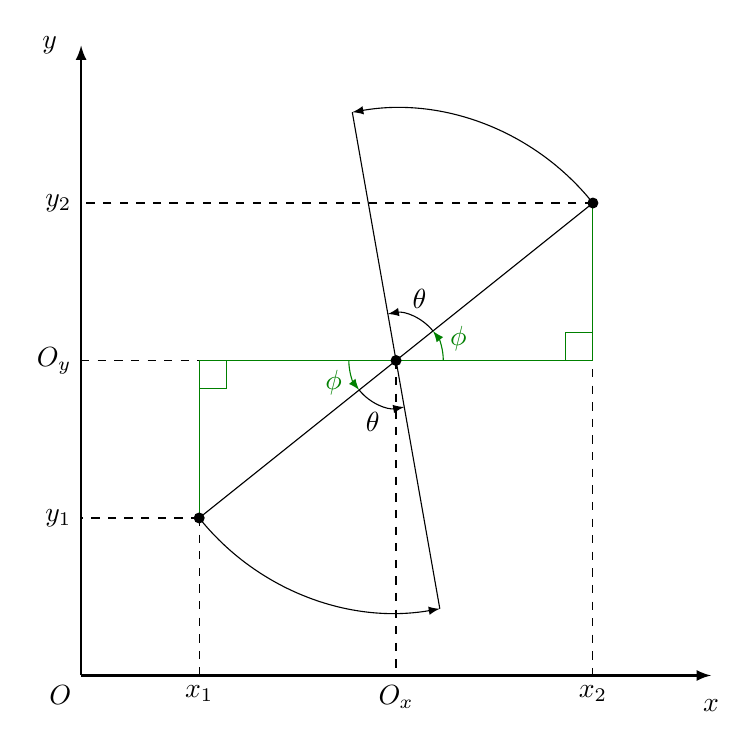
\begin{tikzpicture}
\draw[thick,-latex] (1,1) -- (1,9) node[pos=1,left=5pt] {$y$}; % y-axis
\draw[thick,-latex] (1,1) -- (9,1) node[pos=1,below=5pt] {$x$}; % x-axis
\node[below left] at (1,1) {$O$};
\coordinate (LI) at (2.5,3); % make coordinates for pic right angles
\coordinate (RI) at (7.5,7); % make coordinates for pic right angles
\coordinate (O) at (5,5); % make coordinates for pic right angles
\draw[] (LI) -- (RI); % initial radial line
\coordinate (LG) at (2.5,5); % make coordinates for pic right angles
\coordinate (RG) at (7.5,5); % make coordinates for pic right angles
\coordinate (LF) at (5.5559,1.8471); % coordinate
\coordinate (RF) at (4.4441,8.15292); % coordinate

\draw[] (LF) -- (RF); % final line

\draw[-latex] (LI) arc [start angle=180+38.6598, end angle=280, radius=3.20156]; % left arc
\draw[-latex] (RI) arc [start angle=38.6598, end angle=100, radius=3.20156]; % right arc

%%% ORIGIN DASHES %%%
\draw[dashed] (1,5) -- (5,5);
\node[left] at (1,5) {$O_y$};
\draw[dashed] (5,5) -- (5,1);
\node[below] at (5,1) {$O_x$};

%%% INITIAL DASHES %%%
\draw[dashed] (LI) -- (LI -| 1,0) node[pos=1,left] {$y_1$};
\draw[dashed] (LI) -- (LI |- 0,1) node[pos=1,below] {$x_1$};

%%% FINAL DASHES %%%
\draw[dashed] (RI) -- (RI -| 1,0) node[pos=1,left] {$y_2$};
\draw[dashed] (RI) -- (RI |- 0,1) node[pos=1,below] {$x_2$};


\draw[Green] (LI) -- (LG) -- (RG) -- (RI); % green stuff
\draw pic["$\phi$",-latex,draw,angle eccentricity=1.4, angle radius=0.6cm,Green]{angle=RG--O--RI}; % angle
\draw pic["$\phi$",-latex,draw,angle eccentricity=1.4, angle radius=0.6cm,Green]{angle=LG--O--LI}; % angle
\draw pic["",-,draw,angle eccentricity=1.4, angle radius=0.35cm,Green]{right angle=O--RG--RI}; % angle
\draw pic["",-,draw,angle eccentricity=1.4, angle radius=0.35cm,Green]{right angle=LI--LG--O}; % angle
\draw pic["$\theta$",-latex,draw,angle eccentricity=1.4, angle radius=0.6cm]{angle=RI--O--RF}; % angle
\draw pic["$\theta$",-latex,draw,angle eccentricity=1.4, angle radius=0.6cm]{angle=LI--O--LF}; % angle


%%% MUSTBE ON TOP %%%
\fill[] (O) circle [radius=0.07]; % origin of circle
\fill[] (LI) circle [radius=0.07]; % left point original
\fill[] (RI) circle [radius=0.07]; % right point original
\end{tikzpicture}}
\end{center}
\vspace*{\fill}

\newpage

Where the radial line is of length 1:

\begin{align}
(x_2,y_2)&\longrightarrow(\cos(\phi+\theta)+x_2,\sin(\phi+\theta)+y_2)\\
(x_1,y_1)&\longrightarrow(-\cos(\phi+\theta)+x_1,-\sin(\phi+\theta)+y_1)
\end{align}

\newpage










\topskip0pt
\vspace*{\fill}
\begin{center}
\resizebox{\textwidth}{!}{
\begin{tikzpicture}
\coordinate (O) at (0,0); % origin
\coordinate (L) at (0,5); % height
\coordinate (A) at (10,0); % width
\draw[Blue] (O) -- (L) -- (A) -- cycle; % triangle base
\draw pic["",-,draw,angle eccentricity=1, angle radius=0.5cm,Blue]{right angle=A--O--L}; % right angle
\draw pic["$\theta$",-latex,draw,angle eccentricity=1.4, angle radius=0.8cm,Blue]{angle=O--L--A}; % angle theta
\draw pic["$\frac{\pi}{2}-\theta$",-,draw,angle eccentricity=1.4, angle radius=1.6cm,Blue]{angle=L--A--O}; % calculated angle [(pi/2) - theta]
\draw [decorate,decoration = {brace,mirror},cyan] (0,-0.2) --  (10,-0.2) node[pos=0.5,below=3pt,cyan]{$A$}; % auxillary aid to denote horizontal projection
\draw [decorate,decoration = {brace,},cyan] (-0.2,0) --  (-0.2,5) node[pos=0.5,left=3pt,cyan]{$L$}; % auxillary aid to denote vertical projection
\coordinate (C) at (10,0); % center of unit-circle angle
\coordinate (R) at (13,0); % right of unit-circle angle
\draw[black] (10,0) -- (13,0); % auxillary aid to denote unit-circle angle
\draw pic["\color{red}$\frac{3\pi}{2}+\theta=\arctan(m)\color{black}$",-latex,draw,angle eccentricity=1.4, angle radius=1.6cm]{angle=R--C--L}; % the unit circle angle
\draw[cyan,dashed,->] (0,5) -- (-1.5,5.75) node[pos=0.5,right=1cm]{$\color{cyan}y=\tan\left(\frac{3\pi}{2}-\theta\right)\cdot x+L$}; % left line extension
\draw[cyan,dashed,->] (10,0) -- (12,-1); % right line extension
\end{tikzpicture}}
\end{center}
\vspace*{\fill}

\newpage

\begin{align}
A&=\left(\cos\left(\frac{3\pi}{2}+\theta\right)\right)\cdot\sqrt{A^2+L^2}\\
\therefore\theta(A)&\equiv\arccos\left(\frac{A}{\sqrt{A^2+L^2}}\right)-\frac{3\pi}{2}\\
\therefore y(x)&=\tan\left(\frac{3\pi}{2}-\left(\arccos\left(\frac{A}{\sqrt{A^2+L^2}}\right)-\frac{3\pi}{2}\right)\right)\cdot x+L\\
\mbox{NB:}\ |\theta|&<\frac{\pi}{2}
\end{align}


\newpage

\vspace*{\fill}
\begin{center}
\resizebox{\textwidth}{!}{
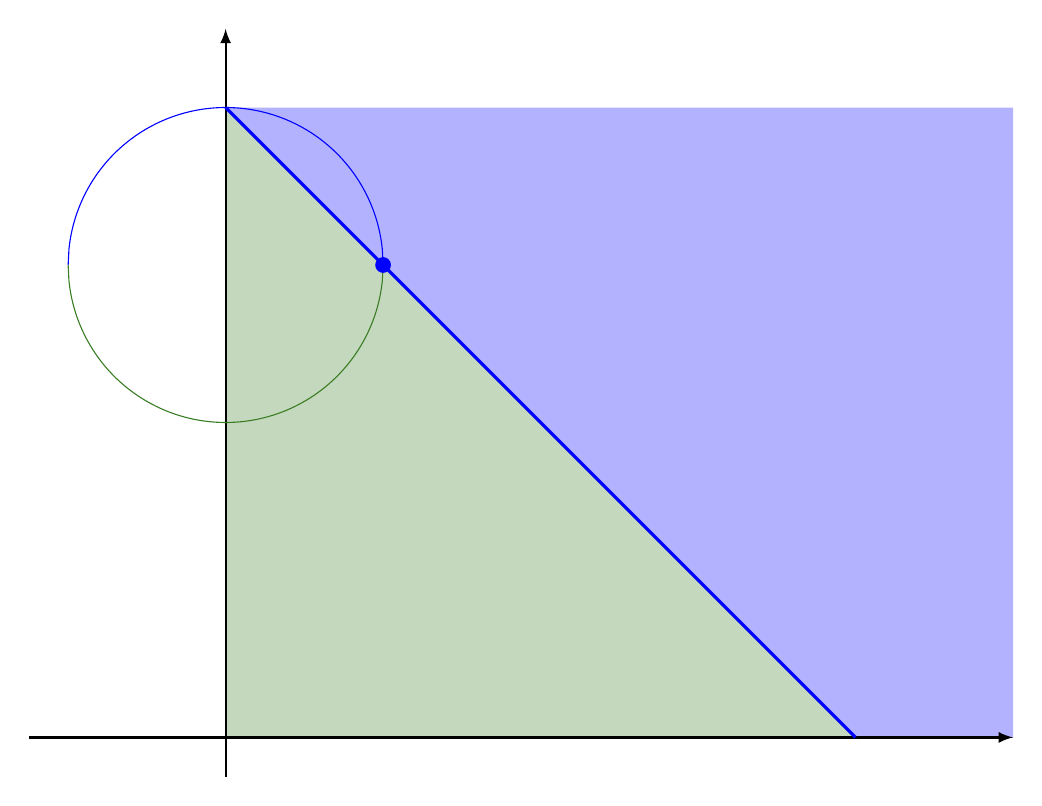
\begin{tikzpicture}
\fill[blue,opacity=0.3] (0,8) -- (8,0) -- (10,0) -- (10,8) -- cycle; % blue shaded area
\fill[OliveGreen,opacity=0.3] (0,0) -- (0,8) -- (8,0) -- cycle; % green shaded area
\draw[black,-latex,thick] (0,-0.5) -- (0,9); % y-axis
\draw[black,-latex,thick] (-2.5,0) -- (10,0); % x-axis
\draw[color=blue,domain=-2:2,samples=400]   plot (\x,{sqrt(4-(\x)^2)+6}); % upper half of circle, inclusive
\draw[color=OliveGreen,domain=-2:2,samples=400]   plot (\x,{-sqrt(4-(\x)^2)+6}); % lower half of circle, exclusive
\draw[color=blue,domain=0:8,very thick]   plot (\x,{-\x+8}); % boundary, blue inclusive
\fill[blue] (2,6) circle [radius=0.1]; % circle boundary, blue inclusive

\end{tikzpicture}}
\end{center}
\vspace*{\fill}

\newpage

\begin{align}
\multicolumn{2}{l}{Per Wolfram$|$Alpha, $x$ for which line=circle is;}\nonumber\\[1em]
x\mbox{-int}_{\mbox{(U\&L)}}(x)&=\frac{2Ar\sqrt{\frac{L^2}{A^2+L^2}}}{\sqrt{A^2+L^2}}
\end{align}


\newpage



\topskip0pt
\vspace*{\fill}
\begin{center}
\resizebox{\textwidth}{!}{
\begin{tikzpicture}
\draw[thick, -latex] (0,-2) -- (0,9); % y-axis
\draw[thick, -latex] (-3,0) -- (11,0); % x-axis
\draw[] (0,4) arc [start angle=-90, end angle=90, radius=2]; % circle right
\draw[dashed] (0,4) arc [start angle=-90, end angle=-270, radius=2]; % circle left
\draw[] (0,8) -- (8,0); % line right
\fill[] (0,8) circle [radius=0.1]; % L
\node[above right] at (0,8) {$L$};
\fill[] (2,6) circle [radius=0.1]; % C-intercept of L
\node[above right] at (2,6) {$I_{L-C}$}; % line-circle intercept
\fill[] (8,0) circle [radius=0.1]; % x-intercept of L
\draw[] (0,6) -- (-2,6); % radius
\draw[decoration={brace,raise=3pt},decorate] (0,6) -- (-2,6) node[pos=0.5, below=5pt]{$r$}; % radius label
\draw[dashed] (0,6) -- (9,6) node[pos=1,right]{$y_{\mbox{int}(L-C)}$}; % y intercept of (line-circle intercept)
\draw[dashed] (2,9) -- (2,0) node[pos=1,below=2pt]{$x_{\mbox{int}(L-C)}$}; % line-axis intercept vertical + label
\fill[] (2,0) circle [radius=0.1]; % line-axis intercept
\node[below=2pt] at (8,0) {$x_{\mbox{int}(L-C)}$}; % line-axis intercept label
\draw[dashed] (0,8) -- (9,8) node[pos=1,right]{$L_y$}; % y-intercept of point L
\node[below=2pt] at (11,0) {$x$}; % x-axis label
\node[left=2pt] at (0,9) {$y$}; % y-axis label
\draw[-latex] (0,7.2) arc [start angle=-90, end angle=-45, radius=0.8]; % angle arc
\node[below right=2pt] at (0.1,7.32) {$\theta$}; % angle denotation - theta
\draw [decorate,decoration = {brace,mirror}] (0,-0.8) --  (8,-0.8) node[pos=0.5,below=3pt]{$a$}; % auxillary aid to denote horizontal projection
\end{tikzpicture}}
\end{center}
\vspace*{\fill}

\newpage

\begin{align}
C(x,\theta)&=\left\{\begin{array}{ll}\sqrt{r^2-x^2}+L_y-r&\mbox{ if } y\geq L_y-r\\-\sqrt{r^2-x^2}+L_y-r&\mbox{ if } y<L_y-r\end{array}\right.\\[2em]
L(x,\theta)&=\left\{\begin{array}{ll}\tan(\theta-\pi)\cdot x+L_y&\mbox{ if } x>0\\\tan(-\theta-\pi)\cdot x+L_y&\mbox{ if } x<0\\
0&\mbox{ if }x=0\end{array}\right.\\[2em]
x_{\mbox{int}(L-C)}(x,\theta)&=\left\{\begin{array}{ll}
\sqrt{\frac{2r(r-\sqrt{r^2-x^2})}{1+\tan(\theta-\pi)}}&\mbox{ if } x\geq0\mbox{ and }y\geq L_y-r\\
-\sqrt{\frac{2r(r-\sqrt{r^2-x^2})}{1+\tan(\theta-\pi)}}&\mbox{ if } x\geq0\mbox{ and }y<L_y-r\\
\multicolumn{2}{l}{\mbox{plus the same sort of equations for x less than zero}}
\end{array}\right.\\[2em]
x_{\mbox{int}(L-\mbox{axis})}(x,\theta)&=\left\{\begin{array}{ll}
-L_y\cot(\theta-\pi)&\mbox{ if } x>0\\
-L_y\cot(-\theta-\pi)&\mbox{ if } x<0\\
0&\mbox{ if }x=0
\end{array}\right.
\end{align}
















\newpage
\topskip0pt
\vspace*{\fill}
\begin{center}
\resizebox{\textwidth}{!}{
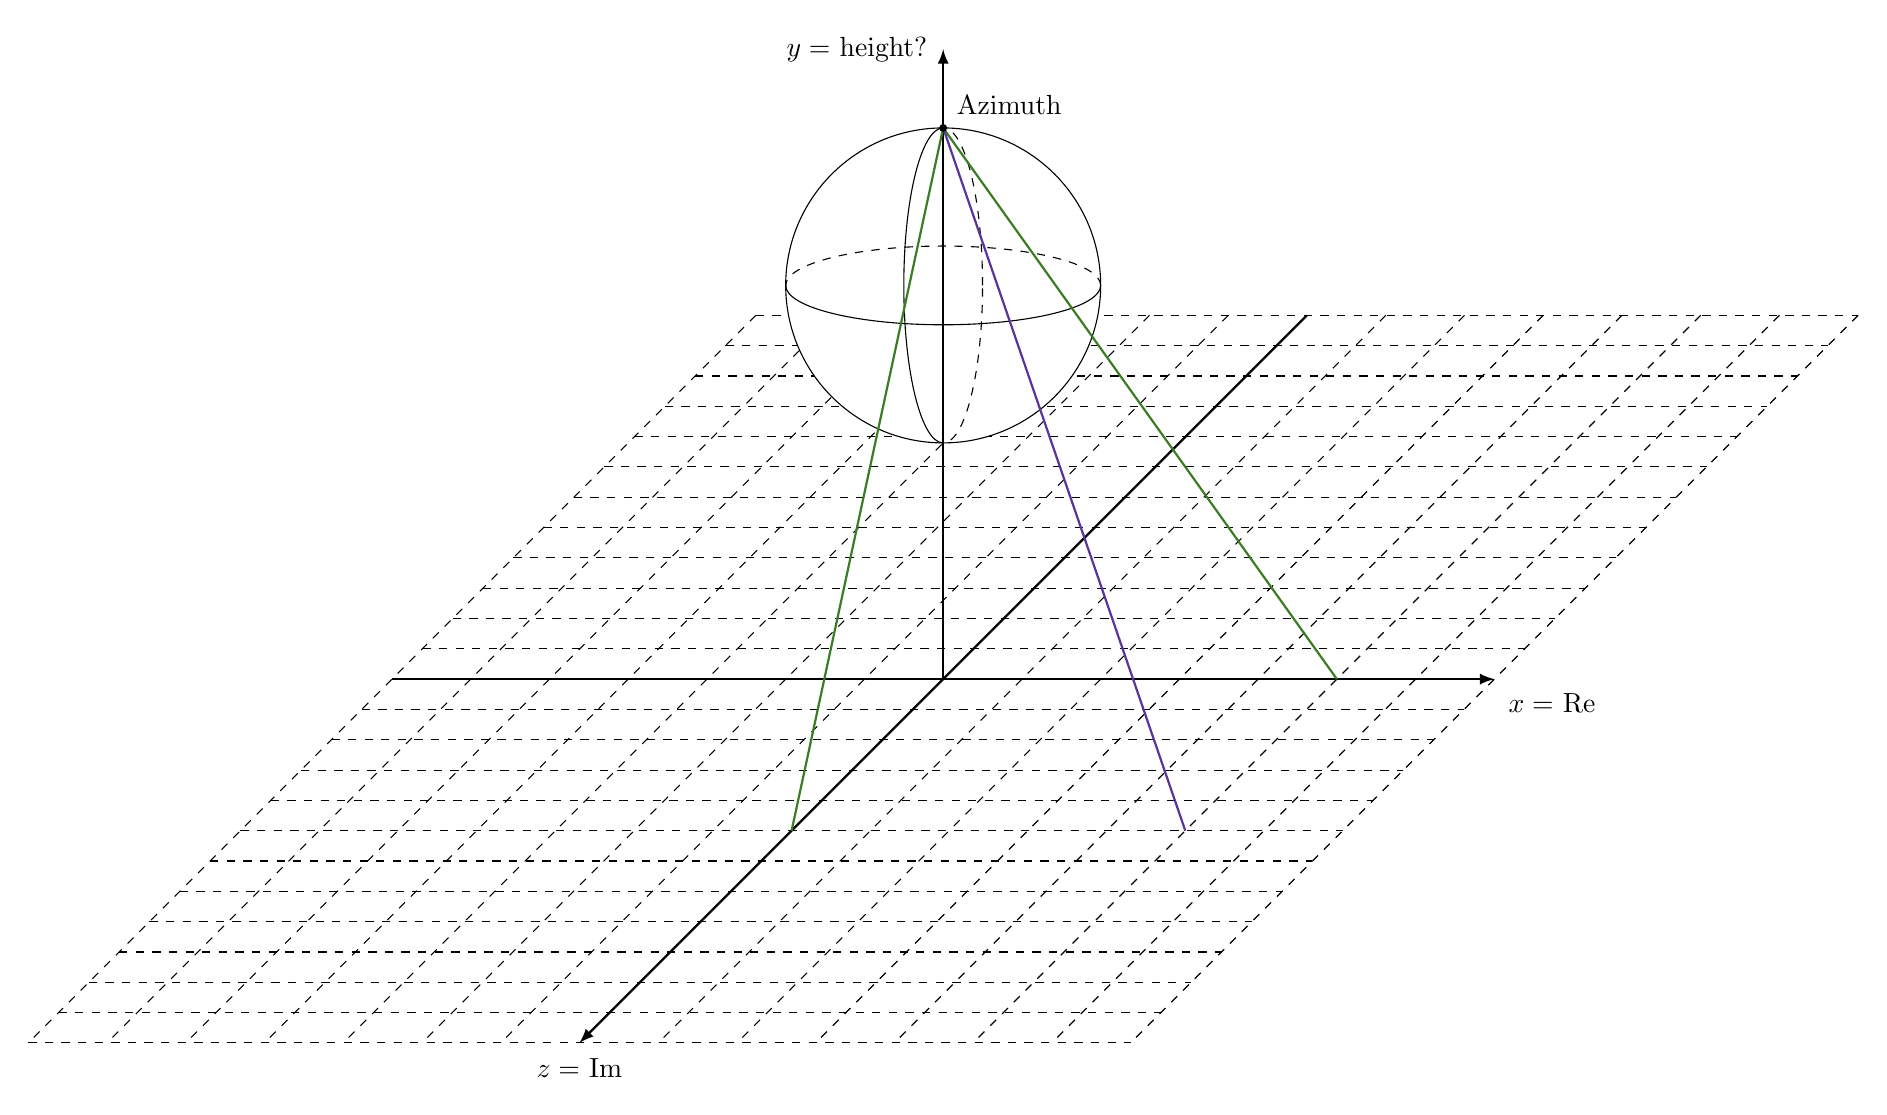
\begin{tikzpicture}

% A path that follows the edges of the current page
\tikzstyle{reverseclip}=[insert path={(current page.north east) --
  (current page.south east) --
  (current page.south west) --
  (current page.north west) --
  (current page.north east)}
]


%%% GRID LINES %%%
\foreach \x in {-7,-6,...,7}{
\draw[dashed] (\x, 0, -12) -- (\x, 0, 12);
}
\foreach \z in {-12,-11,...,12}{
\draw[dashed] (-7, 0, \z) -- (7, 0, \z);
}

\fill[white] (0,5) circle [radius=2];

%%% AXES %%%

%%% x-axis %%%
\draw[thick,-latex] (-7,0,0) -- (7,0,0) node[pos=1,below right=2pt]{$x=$ Re};

%%% y-axis %%%
\draw[thick,-latex] (0,0,0) -- (0,5+3,0) node[pos=1,left=2pt]{$y=$ height?};

%%% z-axis %%%
\draw[thick,-latex] (0,0,-12) -- (0,0,12) node[pos=1,below=2pt]{$z=$ Im};

%%% SPHERE CODE %%%
\draw[] (0,5) circle [radius=2];
\begin{scope} % fix so x>=0
\clip[] (0,-3+5) rectangle (3,3+5);
\draw[dashed] (0,0+5) circle [x radius=0.5, y radius=2];
\end{scope}
\begin{scope} % fix so x<0
\clip[] (0,-3+5) rectangle (-3,3+5);
\draw[] (0, 0+5) circle [x radius=0.5, y radius=2];
\end{scope}
\begin{scope} % fix so y<0
\clip[] (-3,0+5) rectangle (3,-3+5);
\draw[] (0,0+5) circle [x radius=2, y radius=0.5];
\end{scope}
\begin{scope} % fix so y>0
\clip[] (-3,0+5) rectangle (3,3+5);
\draw[dashed] (0,0+5) circle [x radius=2, y radius=0.5];
\end{scope}


%%% RAY TRACES %%%
\draw[OliveGreen,thick] (0,7,0) -- (5,0,0);
\draw[OliveGreen,thick] (0,7,0) -- (0,0,5);
\draw[RoyalPurple,thick] (0,7,0) -- (5,0,5);

%%% THINGS WHICH MUST BE ON TOP %%%
\fill[] (0,7,0) circle [radius=0.05]; % AZIMUTH POINT
\node[above right=2pt] at (0,7,0) {Azimuth};



\end{tikzpicture}}

\end{center}

\vspace*{\fill}




\end{document}